\documentclass[letterpaper]{article}
\usepackage[square,sort,comma,numbers]{natbib}
%====================================================================%
../../../../tex/scufftex.tex

\newcommand\supsstar[1]{^{\hbox{\scriptsize{#1}}*}}
\newcommand\suptstar[1]{^{\hbox{\scriptsize{#1}}*}}
\newcommand{\iD}{_{i\text{\tiny D}}}
\newcommand{\jS}{_{j\text{\tiny S}}}

\newcommand{\OP}{\vb O\sups{power}}
\newcommand{\OG}{\overline{G}}
\newcommand{\SG}{\overline{\vb G}}
\newcommand{\IF}{^{i\text{\scriptsize F}}}
\newcommand{\IT}{^{i\text{\scriptsize T}}}
\newcommand{\lm}{_{\ell m}}
\newcommand{\lmp}{_{\ell^\prime m^\prime}}
\newcommand{\OutD}{^{\hbox{\scriptsize{out}}\dagger}}

\renewcommand{\hslash}{\,\backslash\hspace{-0.06in}h}
\newcommand{\jslash}{\backslash\hspace{-0.05in}j}
\newcommand{\RBar}{\overline{R}}
\newcommand{\RSlash}{\backslash\hspace{-0.08in}R}

\newcommand{\regstar}{^{\hbox{\scriptsize reg}*}}

\graphicspath{{figures/}}

%------------------------------------------------------------
%------------------------------------------------------------
%- Special commands for this document -----------------------
%------------------------------------------------------------
%------------------------------------------------------------

%------------------------------------------------------------
%------------------------------------------------------------
%- Document header  -----------------------------------------
%------------------------------------------------------------
%------------------------------------------------------------
\title {Electromagnetism in the Spherical-Wave Basis: \\
        {\large A (Somewhat Random) Compendium of Reference Formulas}
       }
\author {Homer Reid}
\date {August 1, 2016}

%------------------------------------------------------------
%------------------------------------------------------------
%- Start of actual document
%------------------------------------------------------------
%------------------------------------------------------------

\begin{document}
\pagestyle{myheadings}
\markright{Homer Reid: E\&M in the Spherical-Wave Basis}
\maketitle

\begin{abstract}
This memo consolidates and collects for reference
a somewhat random hodgepodge of formulas and results
in the spherical-wave approach to electromagnetism
that I have found useful over the years in developing
and testing {\sc scuff-em} and {\sc buff-em}.
\end{abstract}

\tableofcontents

%%%%%%%%%%%%%%%%%%%%%%%%%%%%%%%%%%%%%%%%%%%%%%%%%%%%%%%%%%%%%%%%%%%%%%
%%%%%%%%%%%%%%%%%%%%%%%%%%%%%%%%%%%%%%%%%%%%%%%%%%%%%%%%%%%%%%%%%%%%%%
%%%%%%%%%%%%%%%%%%%%%%%%%%%%%%%%%%%%%%%%%%%%%%%%%%%%%%%%%%%%%%%%%%%%%%
\newpage
\section{Vector Spherical Wave Solutions to Maxwell's Equations}
\label{SphericalWaveSection}

Many authors define pairs of three-vector-valued functions
$\{\vb M_{\ell m}(\vb x), \vb N_{\ell m}(\vb x)\}$
describing exact solutions of Maxwell's equations 
in spherical coordinates for 
a homogeneous medium with wavenumber $k$, i.e.
%====================================================================%
$$\Big[\nabla \times \nabla \times - k^2 \Big]
  \left\{\begin{array}{c} \vb M \\ \vb N\end{array}\right\} = 0.$$
%====================================================================%
These functions always involve spherical Bessel functions and
spherical harmonics, but the precise definitions (including
sign conventions and normalization factors) vary from author
to author. In this section I set down the particular
conventions that I use. In the next section I give
explicit closed-form expressions for small $\ell$.

\paragraph{Vector spherical harmonics}
%====================================================================%
\begin{align*}
  \vb X\lm(\theta, \varphi) 
&= \frac{i}{\ell(\ell+1)}\nabla \times 
     \Big\{Y\lm(\theta, \varphi) \vbhat{r}\Big\}
\\
%--------------------------------------------------------------------%
  \vb Z\lm(\theta, \varphi) &= \vbhat{r} \times \vb X\lm(\theta, \varphi)
\end{align*}
%====================================================================%

\noindent More explicitly, the components of $\vb X$ and $\vb Z$ are
%====================================================================%
\begin{align*}
\vb X\lm(\theta, \phi) 
&= 
   \frac{i}{\sqrt{\ell(\ell+1)}}
   \left[  \frac{im}{\sin\theta}Y_{\ell m} \vbhatt{\theta}
           -\pard{Y_{\ell m}}{\theta}\vbhatt{\varphi}
   \right]
\\
\vb Z\lm(\theta, \phi) 
&=
   \frac{i}{\sqrt{\ell(\ell+1)}}
   \left[   \pard{Y_{\ell m}}{\theta}\vbhatt{\theta}
           +\frac{im}{\sin\theta}Y_{\ell m} \vbhatt{\varphi}
   \right].
\end{align*}
%====================================================================%
Their divergences are:
%====================================================================%
\begin{subequations}
\begin{align}
\nabla \cdot \vb X\lm
 &=-\frac{m\cot\theta\csc\theta Y\lm(\theta,\varphi)}
         {r\sqrt{\ell(\ell+1)}}
\\
\nabla \cdot \vb Z\lm
 &= \frac{i\cot\theta}{r \sqrt{\ell(\ell+1)}}
    \Big[ m\cot\theta Y\lm(\theta, \varphi)
          + \xi\lm e^{-i\varphi}Y_{\ell,m+1}(\theta,\varphi)
    \Big]
\\
\xi\lm&\equiv\sqrt\frac{ (\ell-m)! (\ell+m+1)!}{(\ell-m-1)!(\ell+m)!}
\end{align}
\label{XZDivergences}
\end{subequations}
%====================================================================%

\paragraph{Radial functions}
%====================================================================%
\begin{align*}
 R_\ell \sups{outgoing}(kr)  &= h^{(1)}_\ell(kr) \\
 R_\ell \sups{incoming}(kr)  &= h^{(2)}_\ell(kr) \\
 R_\ell \sups{regular}(kr)   &= j_\ell(kr).
\end{align*}
%====================================================================%
I also define the shorthand symbols
%====================================================================%
$$ \RBar_\ell(kr)
   \equiv 
   \frac{1}{kr}\left|R_\ell(x) + \frac{d}{dx}R_\ell(x)\right|_{x=kr}
   \qquad
   \RSlash_\ell(kr) = -\frac{\sqrt{l(l+1)}}{kr} R_\ell(kr).
$$
%====================================================================%

\paragraph{Vector spherical wave functions}
%====================================================================%
\begin{subequations} 
\begin{align} 
 \vb M\lm(k; \vb r) 
&\equiv R_\ell(kr) \vb X\lm(\Omega) 
\\
%--------------------------------------------------------------------%
 \vb N\lm(k; \vb r) &\equiv 
i\RBar_\ell(kr) \vb Z\lm(\Omega) + \RSlash_\ell(kr) Y\lm(\Omega) \vbhat{r} 
\end{align} 
\label{MNDef}%
\end{subequations} 
%====================================================================%

\paragraph{Curl Identities}

$$ \nabla \times \vb M = -ik\vb N, \qquad
   \nabla \times \vb N = +ik\vb M.
$$

\paragraph{General solution of source-free Maxwell equations}

The general solution of Maxwell's equations in a source-free
medium with relative material properties $\epsilon^r, \mu^r$ 
then reads
%====================================================================%
\begin{subequations}
\begin{align}
 \vb E(\vb x)
 &= \hphantom{\frac{1}{Z_0 Z^r}} \sum_\alpha 
     \Big\{ \vb A_\alpha \vb M_\alpha(k; \vb r)
           +\vb B_\alpha \vb N_\alpha(k; \vb r)
     \Big\} 
\\
 \vb H(\vb x)
 &= \frac{1}{Z_0 Z^r} \sum_\alpha 
     \Big\{ \vb B_\alpha \vb M_\alpha(k; \vb r)
           -\vb A_\alpha \vb N_\alpha(k; \vb r)
     \Big\} 
\end{align}
\label{EHExpansion}%%%%
\end{subequations}
%====================================================================%
where $k=\sqrt{\epsilon_0 \epsilon^r \mu_0 \mu^r}\cdot \omega$
is the photon wavenumber in the medium,
$Z_0=\sqrt{\mu_0/\epsilon_0}\sim 377\,\Omega$ is the impedance
of vacuum,
$Z^r=\sqrt{\mu^r/\epsilon^r}$ is the relative wave impedance
of the medium, and we must choose the $\vb M, \vb N$ 
functions to be regular, incoming, or outgoing depending
on the physical conditions of the problem.

%%%%%%%%%%%%%%%%%%%%%%%%%%%%%%%%%%%%%%%%%%%%%%%%%%%%%%%%%%%%%%%%%%%%%%
%%%%%%%%%%%%%%%%%%%%%%%%%%%%%%%%%%%%%%%%%%%%%%%%%%%%%%%%%%%%%%%%%%%%%%
%%%%%%%%%%%%%%%%%%%%%%%%%%%%%%%%%%%%%%%%%%%%%%%%%%%%%%%%%%%%%%%%%%%%%%
\newpage
\section{Explicit expression for small $\ell$}
\label{ExplicitExpressionSection}

\paragraph{The first few radial functions}

%====================================================================%
$$\begin{array}{lclclcl}
% R\sups{regular}_0(kr) 
%&=&
% \displaystyle{ \frac{\sin kr}{kr} }
%&\qquad&
% \displaystyle{ \RBar\sups{regular}_0(kr)  }
%&=&
% \displaystyle{ \frac{i\cos kr}{kr} }
%\\[10pt]
%%--------------------------------------------------------------------%
% R\sups{outgoing}_0(kr) 
%&=&
% \displaystyle{ \frac{-i e^{ikr}}{kr} }
%&\qquad&
% \displaystyle{ \RBar\sups{outgoing}_0(kr) }
%&=&
% \displaystyle{ \frac{ie^{ikr}}{kr} }
%\\[10pt]
%%--------------------------------------------------------------------%
% R\sups{incoming}_0(kr) 
%&=&
% \displaystyle{ \frac{e^{-ikr}}{kr} }
%&\qquad&
% \displaystyle{ \RBar\sups{outgoing}_0(kr) }
%&=&
% \displaystyle{ \frac{e^{-ikr}}{kr} } 
%\\[10pt]
%--------------------------------------------------------------------%
 R\sups{regular}_1(x) 
&=&
 \displaystyle{ -\frac{\cos x}{x} + \frac{\sin x}{x^2} }
&\qquad&
 \displaystyle{ \RBar\sups{regular}_1(x)  }
&=&
 \displaystyle{ \frac{\cos x}{x^2} + \frac{(x^2-1)\sin x}{x^3}
              }
\\[10pt]
%--------------------------------------------------------------------%
 R\sups{outgoing}_1(x) 
&=&
 \displaystyle{ -i\frac{(1-ix)e^{ix}}{x^2}}
&\qquad&
 \displaystyle{ \RBar\sups{outgoing}_1(x) }
&=&
 \displaystyle{ i\frac{(1-ix+x^2)e^{ix}}{x^3} }
\end{array}$$
%====================================================================%

\paragraph{The first few regular functions}

In what follows, the $\zeta_n$ are dimensionless sinusoidal functions:
%====================================================================%
\begin{align*}
 \zeta_1(x) &= \sin x - x \cos x \\
 \zeta_2(x) &= (1-x^2)\sin x - x \cos x
\end{align*}
%====================================================================%

%====================================================================%
\begin{align*}
 \vb M\sups{regular}_{1,\pm 1}(\vb r)
  &=\sqrt\frac{3}{16\pi}\Bf{\zeta_1(kr)}{(kr)^2} e^{\pm i\varphi}
    \left(\begin{array}{c}
    0                 \\
    1                 \\
    \pm i\cos \theta
    \end{array}\right)
\\[5pt]
%--------------------------------------------------------------------%
 \vb M\sups{regular}_{1,0}(\vb r)
  &=\sqrt\frac{3}{8\pi}\Bf{\zeta_1(kr)}{(kr)^2}
    \left(\begin{array}{c}
    0                 \\
    0                 \\
    i\sin \theta
    \end{array}\right)
\\[5pt]
%--------------------------------------------------------------------%
 \vb N\sups{regular}_{1,\pm 1}(\vb r)
  &=\sqrt\frac{3}{16\pi}\Bf{1}{(kr)^3} e^{\pm i\varphi}
    \left(\begin{array}{c}
    \pm 2\zeta_1(kr) \sin \theta \\
    \mp\zeta_2(kr) \cos \theta \\
    -i\zeta_2(kr)
    \end{array}\right)
\\[5pt]
%--------------------------------------------------------------------%
 \vb N\sups{regular}_{1,0}(\vb r)
  &=\frac{1}{2\sqrt{2}(kr)^3}
    \left(\begin{array}{c}
    -2\zeta_1(kr)\cos\theta \\
    -\zeta_2(kr)\sin\theta  \\
    0                
    \end{array}\right)
%--------------------------------------------------------------------%
\end{align*}
%====================================================================%

\paragraph{The first few outgoing functions}

In what follows, the $Q_n$ are dimensionless polynomial factors:
%====================================================================%
\begin{align*}
 Q_1(x) &= 1-x \\
 Q_{2a}(x) &= 1-x+x^2 \\
 Q_{2b}(x) &= 3-3x+x^2 \\
 Q_3(x) &= 6-6x+3x^2-x^3
\end{align*}
%====================================================================%
\begin{align*}
 \vb M\sups{outgoing}_{1,\pm 1}(\vb r)
  &=\sqrt\frac{3}{16\pi}\pf{e^{ikr}}{k^2 r^2} e^{\pm i\phi}
    \left(\begin{array}{c}
    0          \\
    -iQ_1(ikr) \\
    \pm Q_1(ikr) \cos\theta 
    \end{array}\right)
\\[5pt]
%--------------------------------------------------------------------%
 \vb M\sups{outgoing}_{1,0}(\vb r)
  &=\sqrt\frac{3}{8\pi}\pf{e^{ikr}}{k^2 r^2}
    \left(\begin{array}{c}
    0       \\
    0       \\
    Q_1(ikr) \sin\theta 
    \end{array}\right)
\\
%--------------------------------------------------------------------%
 \vb N\sups{outgoing}_{1,\pm 1}(\vb r)
  &=\sqrt\frac{3}{16\pi}\pf{e^{ikr}}{k^3 r^3} e^{\pm i\phi}
    \left(\begin{array}{c}
    \mp -2(ikr)Q_1(ikr)\sin \theta   \\
    \pm iQ_{2a}(ikr) \cos\theta      \\
    -Q_{2a}(ikr)
    \end{array}\right)
\\
%--------------------------------------------------------------------%
 \vb N\sups{outgoing}_{1,0}(\vb r)
  &=\sqrt\frac{3}{8\pi}\pf{e^{ikr}}{k^3 r^3}
    \left(\begin{array}{c}
    2iQ_1(ikr)\cos \theta		\\
    +iQ_{2a}(ikr)\sin\theta	\\
    0
    \end{array}\right)
\\[5pt]
%--------------------------------------------------------------------%
 \vb M\sups{outgoing}_{2,\pm 2}(\vb r)
  &=\sqrt\frac{5}{16\pi}\pf{e^{ikr}}{k^3 r^3} e^{\pm 2i\phi}
    \left(\begin{array}{c}
    0 				  \\
   \pm  iQ_{2b}(ikr)\sin\theta	  \\
    -Q_{2b}(ikr)\cos\theta\sin\theta
    \end{array}\right)
\\
%--------------------------------------------------------------------%
 \vb M\sups{outgoing}_{2,\pm 1}(\vb r)
  &=\sqrt\frac{5}{16\pi}\pf{e^{ikr}}{k^3 r^3} e^{\pm i\phi}
    \left(\begin{array}{c}
    0                            \\
    -iQ_{2b}(ikr)\cos\theta  \\
    \pm Q_{2b}(ikr)\cos 2\theta
    \end{array}\right)
\\
%--------------------------------------------------------------------%
 \vb M\sups{outgoing}_{2,0}(\vb r)
  &=\sqrt\frac{15}{8\pi}\pf{e^{ikr}}{k^3 r^3}
    \left(\begin{array}{c}
    0 \\ 
    0 \\ 
    -Q_{2b}(ikr)\cos \theta \sin\theta
    \end{array}\right)
\\[5pt]
%--------------------------------------------------------------------%
 \vb N\sups{outgoing}_{2,\pm 2}(\vb r)
  &=\sqrt\frac{5}{16\pi}\pf{e^{ikr}}{k^4 r^4} e^{\pm 2i\phi}
    \left(\begin{array}{c}
   3iQ_{2b}(ikr) \sin^2 \theta                          \\
   -iQ_3(ikr) \cos\theta \sin\theta   \\
   \pm Q_3(ikr) \sin\theta 
    \end{array}\right)
\\
%--------------------------------------------------------------------%
 \vb N\sups{outgoing}_{2,\pm 1}(\vb r)
  &=\sqrt\frac{5}{16\pi}\pf{e^{ikr}}{k^4 r^4} e^{\pm i\phi}
    \left(\begin{array}{c}
   \mp 3iQ_{2b}(ikr) \sin 2\theta               \\
   \pm iQ_3(ikr) \cos 2\theta  \\
   -Q_3(ikr) \cos\theta
    \end{array}\right)
\\
%--------------------------------------------------------------------%
 \vb N\sups{outgoing}_{2,0}(\vb r)
  &=\sqrt\frac{15}{8\pi}\pf{e^{ikr}}{k^4 r^4}
    \left(\begin{array}{c}
   iQ_{2b}(ikr)(3\cos^2 \theta -1)                    \\
   iQ_3(ikr) \cos \theta \sin\theta \\
   0
    \end{array}\right).
\end{align*}

%%%%%%%%%%%%%%%%%%%%%%%%%%%%%%%%%%%%%%%%%%%%%%%%%%%%%%%%%%%%%%%%%%%%%%
%%%%%%%%%%%%%%%%%%%%%%%%%%%%%%%%%%%%%%%%%%%%%%%%%%%%%%%%%%%%%%%%%%%%%%
%%%%%%%%%%%%%%%%%%%%%%%%%%%%%%%%%%%%%%%%%%%%%%%%%%%%%%%%%%%%%%%%%%%%%%
\newpage
\section{Translation matrices}
\label{TranslationMatrixSection}

Translation matrices arise when we want to evaluate the fields
produced by sources not located at the origin. 

\paragraph{Scalar case}
Although we don't need it for electromagnetism problems,
the scalar-wave analog of (\ref{MNDef}) is
%%%%%%%%%%%%%%%%%%%%%%%%%%%%%%%%%%%%%%%%%%%%%%%%%%%%%%%%%%%%%%%%%%%%%%
$$ \psi\lm(\vb x) = R_\ell(kr)Y\lm(\theta,\phi)$$
%%%%%%%%%%%%%%%%%%%%%%%%%%%%%%%%%%%%%%%%%%%%%%%%%%%%%%%%%%%%%%%%%%%%%%
or, more specifically,
%%%%%%%%%%%%%%%%%%%%%%%%%%%%%%%%%%%%%%%%%%%%%%%%%%%%%%%%%%%%%%%%%%%%%%
$$ \psi\lm\sups{out}(\vb x) = R_\ell\sups{out}(kr)Y\lm(\theta,\phi),
   \qquad
   \psi\lm\sups{reg}(\vb x) = R_\ell\sups{reg}(kr)Y\lm(\theta,\phi)
$$
%%%%%%%%%%%%%%%%%%%%%%%%%%%%%%%%%%%%%%%%%%%%%%%%%%%%%%%%%%%%%%%%%%%%%%
Now consider a point source at $\vb x\supt{S}$ whose fields we wish
to evaluate at an evaluation (``destination'') point $\vb x\supt{D}$,
using a basis of spherical waves centered at an origin $\vb x\supt{O}$.
Then waves emitted by the source, which appear to be outgoing in a
coordinate system centered at $\vb x\supt{S}$, can be described
as superpositions of regular waves in a coordinate system
centered at $\vb x\supt{O}$:
%%%%%%%%%%%%%%%%%%%%%%%%%%%%%%%%%%%%%%%%%%%%%%%%%%%%%%%%%%%%%%%%%%%%%%
\numeq{ScalarTranslationFormula}
{ \psi\sups{out}_\alpha\big(\vb x\supt{D}-\vb x\supt{S}\big)
   =\sum_\beta A_{\alpha\beta}\big(k; \vb x\supt{S} - \vb x\supt{O}\big)
               \psi\sups{reg}_\beta\big( \vb x\supt{D}-\vb x\supt{O}\big)
}
where $\alpha,\beta$ are compound indices 
(i.e. $\alpha=\{\ell_\alpha, m_\alpha\}$) and 
%%%%%%%%%%%%%%%%%%%%%%%%%%%%%%%%%%%%%%%%%%%%%%%%%%%%%%%%%%%%%%%%%%%%%%
\begin{align*}
 A_{\alpha\beta}(k, \vb L)
&=4\pi 
  \sum_\gamma i^{(\ell_\alpha - \ell_\beta + \ell_\gamma)}
  a_{\alpha\gamma\beta} 
  \psi\sups{out}_\gamma(\vb L)
\\
a_{\alpha\beta\gamma}
&=\int Y_\alpha(\Omega) Y^*_\beta(\Omega) Y^*_\gamma(\Omega) \, d\Omega
\\
&=(-1)^{m_\alpha}
  \sqrt\frac{ (2\ell_\alpha+1)(2\ell_\beta+1) (2\ell_\gamma+1)}
            {4\pi}
  \left(\begin{array}{ccc} 
        \ell_\alpha & \ell_\beta & \ell_\gamma \\ 0 & 0 & 0 
        \end{array}\right)
  \left(\begin{array}{ccc} 
        \ell_\alpha & \ell_\beta & \ell_\gamma \\ 
          -m_\alpha & m_\beta    & m_\gamma
        \end{array}\right).
\end{align*}
%%%%%%%%%%%%%%%%%%%%%%%%%%%%%%%%%%%%%%%%%%%%%%%%%%%%%%%%%%%%%%%%%%%%%%

\paragraph{Vector case}

%%%%%%%%%%%%%%%%%%%%%%%%%%%%%%%%%%%%%%%%%%%%%%%%%%%%%%%%%%%%%%%%%%%%%%
\begin{align*}
 \left(\begin{array}{c}
   \vb M \\ \vb N
 \end{array}\right)\sups{out}_\alpha
&= 
 \sum_{\beta}
 \left(\begin{array}{cc}
   \vb B & \vb C \\ 
  -\vb C & \vb B
 \end{array}\right)_{\alpha\beta} 
 \left(\begin{array}{c}
   \vb M \\ \vb N 
 \end{array}\right)\sups{reg}_\beta
\end{align*}
%%%%%%%%%%%%%%%%%%%%%%%%%%%%%%%%%%%%%%%%%%%%%%%%%%%%%%%%%%%%%%%%%%%%%%

%%%%%%%%%%%%%%%%%%%%%%%%%%%%%%%%%%%%%%%%%%%%%%%%%%%%%%%%%%%%%%%%%%%%%%
\begin{align*}
 B_{\alpha\beta}(k, \vb L)
&=4\pi 
  \sum_\gamma i^{(\ell_\alpha - \ell_\beta + \ell_\gamma)}
  \left[\frac{\ell_\alpha(\ell_\alpha + 1) + \ell_\beta(\ell_\beta + 1) 
               -\ell_\gamma(\ell_\gamma+ 1)
             }
             {2\sqrt{\ell_\alpha(\ell_\alpha+1)\ell_\beta (\ell_\beta+1)}}
  \right]
  a_{\alpha\gamma\beta} 
  \psi\sups{out}_\gamma(\vb L)
\\
 C_{\alpha\beta}(k, \vb L)
&=-\frac{k}{\sqrt{\ell_\alpha(\ell_\alpha+1)\ell_\beta(\ell_\beta+1)}}
   \left[ \frac{\lambda_+}{2}\big(L_x - iL_y\big)A_{\alpha_+, \beta} 
         +\frac{\lambda_-}{2}\big(L_x + iL_y\big)A_{\alpha_-, \beta} 
         +           m_\alpha L_z A_{\alpha, \beta} 
   \right]
\end{align*}
$$ \lambda_\pm = \sqrt{ (\ell_\alpha \mp \ell_\beta)
                        (\ell_\alpha \pm \ell_\beta+1)
                      },
   \qquad
   \alpha_\pm = \{\ell_\alpha, m_\alpha \pm 1\}
$$

%%%%%%%%%%%%%%%%%%%%%%%%%%%%%%%%%%%%%%%%%%%%%%%%%%%%%%%%%%%%%%%%%%%%%%
%%%%%%%%%%%%%%%%%%%%%%%%%%%%%%%%%%%%%%%%%%%%%%%%%%%%%%%%%%%%%%%%%%%%%%
%%%%%%%%%%%%%%%%%%%%%%%%%%%%%%%%%%%%%%%%%%%%%%%%%%%%%%%%%%%%%%%%%%%%%%
\newpage
\section{Spherical-wave expansion of incident fields}

\subsection{Plane waves}
\label{PlaneWaveSection}

For a scattering problem in which the incident field
is a $z$-directed plane wave, i.e.
%====================================================================%
$$
 \vb E\sups{inc}=\vb E_0e^{ik z}, \qquad 
 \vb H\sups{inc}=\frac{1}{Z_0}\vbhat{z}\times \vb E_0 e^{ik z}
$$
%====================================================================%
the spherical-wave expansion coefficients in (\ref{EHIncOutsideExpansion})
take the following forms for various possible polarizations:
%====================================================================%
$$\begin{array}{rclll}
\vb E_0 &=& \vbhat{x} + i\vbhat{y} 
 \quad &\text{(right circular polarization)}:
 \qquad &P\lm=\delta_{m,+1}P_\ell
\\[5pt]
\vb E_0 &=& \vbhat{x} - i\vbhat{y} 
 \quad &\text{(left circular polarization)}:
 \qquad &P\lm=\delta_{m,-1}P_\ell 
\\[3pt]
\vb E_0 &=& \vbhat{x}
 \quad &\text{(linear polarization)}:
 \qquad &P\lm=\frac{1}{2}\Big(\delta_{m,+1} + \delta_{m,-1}\Big)P_\ell 
\end{array}$$
%====================================================================%
where in all cases I have
%====================================================================%
$$ P_\ell = i^\ell \sqrt{4\pi(2\ell +1)}, \qquad  
   Q_{\ell, \pm 1} = \mp i P_\ell.
$$
%====================================================================%

%%%%%%%%%%%%%%%%%%%%%%%%%%%%%%%%%%%%%%%%%%%%%%%%%%%%%%%%%%%%%%%%%%%%%%
%%%%%%%%%%%%%%%%%%%%%%%%%%%%%%%%%%%%%%%%%%%%%%%%%%%%%%%%%%%%%%%%%%%%%%
%%%%%%%%%%%%%%%%%%%%%%%%%%%%%%%%%%%%%%%%%%%%%%%%%%%%%%%%%%%%%%%%%%%%%%
\subsection{Point sources at the origin}
\label{PointSourceAtOriginSection}

Let $\vb E(\vb x; \vb p)$ be the electric field
at evaluation point $\vb x$ due to an electric dipole
$\vb p$ at the origin. The spherical-wave expansion
of this field involves only $\vb N$-functions
with $\ell=1$, i.e.
%====================================================================%
$$ \vb E(\vb x; \vb p) = 
   \sum_{m=-1}^1 \xi_{1m}(\vb p) \vb N_{1m}\sups{outgoing}(\vb x)
$$
%====================================================================%
where the $\xi$ coefficients are
%====================================================================%
$$\begin{array}{clll}
\vb p=p_x \vbhat{x}
&\qquad\longrightarrow\qquad
&\displaystyle{
  \xi_{1,1}=-\xi_{1,-1}=\frac{i}{2}\frac{k^3}{\sqrt{3\pi}}\frac{p_x}{\epsilon},
              }
&\qquad\xi_{1,0}=0
\\[10pt]
\vb p=p_y \vbhat{y}
&\qquad\longrightarrow\qquad
&\displaystyle{
 \xi_{1,1}=+\xi_{1,-1}=\frac{1}{2}\frac{k^3}{\sqrt{3\pi}}\frac{p_y}{\epsilon}
              }
&\qquad\xi_{1,0}=0
\\[10pt]
\vb p=p_z \vbhat{z}
&\qquad\longrightarrow\qquad
&\displaystyle{
 \xi_{1,1}=\xi_{1,-1}=0, 
              } 
&\qquad \xi_{1,0} = 
  \displaystyle{ -\frac{ik^3}{\sqrt{6\pi}} \frac{p_z}{\epsilon} }
\end{array}$$
%====================================================================%
Here $\epsilon=\epsilon_0\epsilon^r$ is the absolute permittivity
of the medium.

Similarly, the magnetic fields of a magnetic dipole $\vb m$ at the
origin are
$$ \vb H(\vb x; \vb m)=\sum_\alpha \wh{\xi}_\alpha(\vb m) \vb N\sups{outgoing}_\alpha(\vb x)
$$
where the $\wh{\xi}$ coefficients are the same as the
$\xi$ coefficients above with the replacement
$\frac{p}{\epsilon} \to \frac{m}{\mu}.$

%=================================================
%=================================================
%=================================================
\subsection{Point sources not at the origin}
\label{PointSourceSection}

The fields of point sources \textit{not} at the
origin may be obtained by applying the translation matrices
of Section \label{TranslationMatrixSection}
to the fields of Section \ref{PointSourceAtOriginSection}.
If the point source lies at $\vb x\supt{S}\ne 0$ (here ``S''
stands for ``source''), then 
its fields at destination point $\vb x\supt{D}$
read
%====================================================================%
\begin{subequations}
\begin{align}
 \vb E(\vb x\supt{D}; \vb x\supt{S}, \vb p)
   &= \sum_{\alpha\beta}
      \Big\{
       -\xi_\alpha C_{\alpha\beta}  \vb M_\beta\sups{regular}(\vb x\supt{D})
       +\xi_\alpha B_{\alpha\beta} \vb N_\beta\sups{regular}(\vb x\supt{D})
      \Big\}
\\
 \vb H(\vb x\supt{D}; \vb x\supt{S}, \vb p)
   &= \frac{1}{Z}\sum_{\alpha\beta}
                    \Big\{
         \xi_\alpha C_{\alpha\beta} \vb N_\beta\sups{regular}(\vb x\supt{D})
       + \xi_\alpha B_{\alpha\beta} \vb M_\beta\sups{regular}(\vb x\supt{D})
                    \Big\}
\\[10pt]
 \vb E(\vb x\supt{D}; \vb x\supt{S}, \vb m)
   &=-Z \sum_{\alpha\beta} \Big\{
        \wh{\xi}_\alpha B_{\alpha\beta} \vb M_\beta\sups{regular}(\vb x\supt{D})
       +\wh{\xi}_\alpha C_{\alpha\beta} \vb N_\beta\sups{regular}(\vb x\supt{D})
                    \Big\}
\\
 \vb H(\vb x\supt{D}; \vb x\supt{S}, \vb m)
   &= \sum_{\alpha\beta} \Big\{
       -\wh{\xi}_\alpha C_{\alpha\beta} \vb M_\beta\sups{regular}(\vb x\supt{D})
       +\wh{\xi}_\alpha B_{\alpha\beta} \vb N_\beta\sups{regular}(\vb x\supt{D})
                    \Big\}
\end{align}
\label{TranslatedPSFields}
\end{subequations}
%====================================================================%
Here $\{B,C\}_{\alpha\beta}$ are elements of the translation matrices
$\vb B(k,\vb x\supt{S}), \vb C(k,\vb x\supt{S}).$

Note that, for a given source point $\vb x\supt{S}$, I only have
to assemble the translation matrices $\vb B$ and $\vb C$ once
(at a given frequency), after which I can get the fields
at any number of destination points $\vb x\supt{D}$ from
equation (\ref{TranslatedPSFields}).


%%%%%%%%%%%%%%%%%%%%%%%%%%%%%%%%%%%%%%%%%%%%%%%%%%%%%%%%%%%%%%%%%%%%%%
%%%%%%%%%%%%%%%%%%%%%%%%%%%%%%%%%%%%%%%%%%%%%%%%%%%%%%%%%%%%%%%%%%%%%%
%%%%%%%%%%%%%%%%%%%%%%%%%%%%%%%%%%%%%%%%%%%%%%%%%%%%%%%%%%%%%%%%%%%%%%
\newpage
\section{Scattering from a homogeneous dielectric sphere}
\label{DielectricSphereScatteringSectionl}

I consider scattering from a single homogeneous sphere
with relative permittivity and permeability $\epsilon^r, \mu^r$
in vacuum
irradiated by spherical waves emanating from within our
outside the sphere.

Irrespective of the origin of the incident fields, 
the scattered fields inside and outside the sphere
take the form ($n=\sqrt{\epsilon^r \mu^r}, Z^r=\sqrt{\mu^r / \epsilon^r})$
%====================================================================%
\paragraph{Inside the sphere:} 
\begin{subequations}
\begin{align}
 \vb E\sups{scat}(\vb x)
 &=\hphantom{\frac{1}{Z_0 Z^r}}  \sum_\alpha 
     \Big\{ A_\alpha \vb M_\alpha\sups{reg}(nk_0; \vb r)
        +   B_\alpha \vb N_\alpha\sups{reg}(nk_0; \vb r)
     \Big\} 
\\
 \vb H\sups{scat}(\vb x)
 &= \frac{1}{Z_0 Z^r} \sum_\alpha 
     \Big\{ B_\alpha \vb M_\alpha\sups{reg}(nk_0; \vb r)
           -A_\alpha \vb N_\alpha\sups{reg}(nk_0; \vb r)
     \Big\} 
\end{align}
\label{EHScatInside}
\end{subequations}
\paragraph{Outside the sphere:} 
\begin{subequations}
\begin{align}
 \vb E\sups{scat}(\vb x)
 &=\hphantom{\frac{1}{Z_0}}  \sum_\alpha 
      \Big\{ C_\alpha \vb M_\alpha\sups{out}(k_0; \vb r)
            +D_\alpha \vb N_\alpha\sups{out}(k_0; \vb r)
      \Big\} 
\\
 \vb H\sups{scat}(\vb x)
 &=  \frac{1}{Z_0} \sum_\alpha 
     \Big\{ D_\alpha \vb M_\alpha\sups{out}(k_0; \vb r)
           -C_\alpha \vb N_\alpha\sups{out}(k_0; \vb r)
     \Big\} 
\end{align}
\label{EHScatOutside}%
\end{subequations}
%====================================================================%
The $\{A, B, C, D\}$ coefficients are proportional to the 
spherical-wave expansion coefficients of the incident fields,
with the proportionality constants determined by enforcing
continuity of the tangential components of the total 
fields $\{\vb E, \vb H\}\sups{tot}=
\{\vb E, \vb H\}\sups{inc}+
\{\vb E, \vb H\}\sups{scat}$
at $r=r_0$,
%====================================================================%
\begin{subequations}
\begin{align}
 \Big| \vbhat{r} \times \vb E\sups{tot} \Big|_{r\to r_0^+}
&=
 \Big| \vbhat{r} \times \vb E\sups{tot} \Big|_{r\to r_0^-}
\\[5pt]
 \Big| \vbhat{r} \times \vb H\sups{tot} \Big|_{r\to r_0^+}
&=
 \Big| \vbhat{r} \times \vb H\sups{tot} \Big|_{r\to r_0^-}
\end{align}
\label{EHMatching}%
\end{subequations}
%====================================================================%

%=================================================
%=================================================
%=================================================
\subsection{Sources outside the sphere}
\label{SourcesOutsideSection}

If the sources of the incident field lie outside the sphere
(the usual Mie scattering problem),
then I can expand the incident fields in the form
%====================================================================%
\begin{subequations}
\begin{align}
  \vb E\sups{inc}(\vb x) =
   \sum_{\alpha}
    \Big\{
        P_\alpha \vb M\sups{regular}_\alpha(k_0; \vb x)
       +Q_\alpha \vb N\sups{regular}_\alpha(k_0; \vb x)
    \Big\}
\\
  \vb H\sups{inc}(\vb x) =
   \frac{1}{Z_0}
   \sum_{\alpha}
    \Big\{
        Q_\alpha \vb M\sups{regular}_\alpha(k_0; \vb x)
       -P_\alpha \vb N\sups{regular}_\alpha(k_0; \vb x)
    \Big\}.
\end{align}
\label{EHIncOutsideExpansion} %
\end{subequations}
%====================================================================%
Matching tangential fields at the sphere surface then 
determines
the scattered-field expansion coefficients in terms of the 
incident-field expansion coefficients $(a=k_0 r_0)$:
%====================================================================%
\begin{subequations}
\begin{align}
 A_\alpha 
 &= \left[\frac{  R\sups{reg}(a) \RBar\sups{out}(a)
                -\RBar\sups{reg}(a) R\sups{out}(a)
         }
         {
            R\sups{reg}(n a) \RBar\sups{out}(a) 
           -\frac{1}{Z^r} \RBar\sups{reg}(n a) R\sups{out}(a)
          }
    \right]P_\alpha
\\
 B_\alpha 
 &= \left[\frac{  \RBar\sups{reg}(a) R\sups{out}(a) 
                -R\sups{reg}(a) \RBar\sups{out}(a)
         }
         {
            \RBar\sups{reg}(n a) R\sups{out}(a) 
           -\frac{1}{Z^r} R\sups{reg}(n a) \RBar\sups{out}(a)
          }
    \right]Q_\alpha
\\[10pt]
 C_\alpha 
 &=\underbrace{ 
    \left[\frac{      R\sups{reg}(a) \RBar\sups{reg}(n a)
                 -Z^r \RBar\sups{reg}(a) R\sups{reg}(n a)
               }
         {
            Z^r R\sups{reg}(n a) \RBar\sups{out}(a) 
           -    \RBar\sups{reg}(n a) R\sups{out}(a)
          }
    \right] }_{\mb T_{\alpha}\supt{M}}
          P_\alpha
\\[8pt]
 D_\alpha 
 &= \underbrace{
    \left[\frac{     \RBar\sups{reg}(a) R\sups{reg}(na) 
                 -Z^r R\sups{reg}(a) \RBar\sups{reg}(na)
         }
         {
            Z^r \RBar\sups{reg}(n a) R\sups{out}(a) 
           - R\sups{reg}(n a) \RBar\sups{out}(a)
          }
    \right]
              }_{\mb T_{\alpha}\supt{N}}
          Q_\alpha
\end{align}
\label{ABCDOutside}%
\end{subequations}
%====================================================================%
In (\ref{ABCDOutside}c,d) I have identified
the quantities $C_\alpha/P_\alpha$ and $D_\alpha/Q_\alpha$
as elements of the $\mb T$-matrix for the $M$- and $N$- 
polarizations.\footnote{The $\mb T$-matrix multiplies a vector
of regular-wave incident-field coefficients to yield 
a vector of outgoing-wave scattered-field coefficients.
If, instead of the regular-wave incident field 
(\ref{EHIncOutsideExpansion}), I irradiated the sphere with
a superposition of \textit{incoming} waves as the incident field,
then the resulting modified versions of equations (\ref{ABCDOutside}c,d)
would instead define elements of the $\mb S$-matrix (scattering matrix).}

\subsubsection{Analytical results in the low-frequency limit}

The coefficients (\ref{ABCDOutside}) may be expressed in closed form, e.g.
%%%%%%%%%%%%%%%%%%%%%%%%%%%%%%%%%%%%%%%%%%%%%%%%%%%%%%%%%%%%%%%%%%%%%%
\begin{align*}
 \frac{A_1}{P_1}
&=
   \frac{2 a^3 e^{-i a} n^3 Z}{\left((1-i a) \left(a^2 n^2-1\right)-(-1+a (a+i))
    n Z\right) \sin (a n)+a n ((-1+a (a+i)) n Z-i a+1) \cos (a n)}
\\
 \frac{B_1}{Q_1}
&=
  \frac{2 a^3 e^{-i a} n^3 Z}{\left((1-i a) Z \left(a^2 n^2-1\right)-(-1+a
    (a+i)) n\right) \sin (a n)+a n ((-1+a (a+i)) n-i a Z+Z) \cos (a n)}
\end{align*}
%%%%%%%%%%%%%%%%%%%%%%%%%%%%%%%%%%%%%%%%%%%%%%%%%%%%%%%%%%%%%%%%%%%%%%
where $a=(k_0 r_0)$ is the dimensionless Mie size parameter.
The low-frequency limiting forms (assuming $\mu=1$:) are 
%%%%%%%%%%%%%%%%%%%%%%%%%%%%%%%%%%%%%%%%%%%%%%%%%%%%%%%%%%%%%%%%%%%%%%
$$ \begin{array}{lclclcl}
 \displaystyle{
 \frac{A_1}{P_1}
              }
&=& 
 \displaystyle{
   \frac{2}{\sqrt{\epsilon}}
   +
   \Big[\frac{(\epsilon-1)}{3\sqrt{\epsilon}}\Big] a^2
   +O(a^3)
              }
&\quad&
 \displaystyle{
 \frac{B_1}{Q_1}
              }
&=& 
 \displaystyle{
    \frac{6}{\epsilon+2}
   +
   \Big[
   \frac{3 \left(\epsilon^2+9\epsilon-10\right)}{5 (\epsilon+2)^2}
   \Big]a^2
   +O(a^3)
              }
\\[12pt]
 \displaystyle{
\frac{A_2}{P_2}
              }
&=&
 \displaystyle{
   \frac{2}{\epsilon}
   +\left[ \frac{(\epsilon-1)}{5\epsilon}\right]a^2
   +O(a^3)
              }
&\quad&
 \displaystyle{
\frac{B_2}{Q_2}
              }
&=&
 \displaystyle{
   \frac{10}{\sqrt{\epsilon} (2 \epsilon+3)}
  +
   \left[ \frac{5 a^2 \left(2\epsilon^2+5 \epsilon-7\right)}
               {7 \sqrt{\epsilon} (2 \epsilon+3)^2}
   \right] a^2 
  +O(a^3)
              }
\end{array}$$

\subsubsection*{Interior fields }

For a sphere irradiated by a linearly-polarized plane wave,
the fields inside the body to second order in $a=kR$ read
%====================================================================%
\begin{align*}
 \frac{E_x}{E_0} &= \frac{3}{2+\epsilon} 
        +\left[\frac{\epsilon+4}{3+2\epsilon}\right] ikz
  +\left[\frac{(\epsilon-1)(35\epsilon+46)}
              {5(\epsilon+2)^2 (3 \epsilon+4)}
   \right]k^2 x^2
\\[5pt]
&\qquad
  +\left[\frac{(\epsilon-1)(-2\epsilon^2+29\epsilon+42)}
              {5(\epsilon+2)^2 (3 \epsilon+4)}
   \right]k^2 y^2
  -\left[\frac{14\epsilon^3 + 3\epsilon^2 + 114\epsilon + 184}
              {10(\epsilon+2)^2 (3 \epsilon+4)}
   \right]k^2 z^2
\\[5pt]
 \frac{E_y}{E_0} 
 &= \left[\frac{2(\epsilon^2-1)}{5(2+\epsilon)(4+3\epsilon)}\right] k^2 xy
\\
 \frac{E_z}{E_0} &= -\left[\frac{\epsilon-1}{2\epsilon+3}\right] ikx
        +\left[\frac{(\epsilon-1)(7\epsilon+12)}
                    {5(2+\epsilon)(4+3\epsilon)}
        \right]k^2 xz
\\[5pt]
 \frac{H_x}{Z_0 E_0} 
 &= \left[\frac{(\epsilon-1)^2}{5(2\epsilon+3)}\right] k^2 xy
\\[5pt]
 \frac{H_y}{Z_0 E_0} 
  &= 1 + \left[\frac{2\epsilon+1}{2+\epsilon}\right] ikz
\\[5pt]
&\qquad - \left[\frac{(\epsilon-1)(\epsilon-6)}{15(3+2\epsilon)}\right]k^2 x^2
        + \left[\frac{\epsilon-1}{15}\right]k^2 y^2 
        - \left[\frac{2\epsilon^2 + 46\epsilon + 27}{30(3+2\epsilon)}
          \right]k^2 z^2
\\
 \frac{H_z}{Z_0 E_0} 
     &= -\left[\frac{\epsilon-1}{\epsilon+2}\right] iky
        +\left[\frac{(\epsilon-1)(\epsilon+4)}
                    {5(3+2\epsilon)}\right] k^2 yz
\end{align*}
%====================================================================%

Field derivatives:
\begin{align*}
 \partial_z \vb E &= \big(ikC_1 - 2k^2 C_2 z\big)\vbhat{x} 
                     +k^2 C_3 x\,\vbhat{z}
\\
 \partial_z \vb H &= \big(ik C_4 - 2k^2 C_5 z\big) \vbhat{y}
                     +k^2 C_6 y\,\vbhat{z}
\end{align*}
\begin{align*}
 C_1 &= \frac{\epsilon+4}{3+2\epsilon},
\\
 C_2 &= \frac{14\epsilon^3 + 3\epsilon^2 + 114\epsilon + 184}
             {10(\epsilon+2)^2 (3 \epsilon+4)}
\\
 C_3 &= \frac{(\epsilon-1)(7\epsilon+12)}{5(2+\epsilon)(4+3\epsilon)}
\\
C_4 &= \frac{2\epsilon+1}{2+\epsilon}
\\
C_5 &= \frac{2\epsilon^2 + 46\epsilon + 27}{30(3+2\epsilon)}
\\
C_6 &= \frac{(\epsilon-1)(\epsilon+4)} {5(3+2\epsilon)}
\end{align*}

%=================================================
%=================================================
%=================================================
\subsection{Sources inside the sphere}

If the sources of the incident field lie inside the sphere,
then I can expand the incident field in the form
%====================================================================%
\numeq{EIncExpansion}
{\vb E\sups{inc}(\vb x) =
   \sum_{\alpha}
    \Big\{
        P_\alpha \vb M\sups{out}_\alpha(nk_0; \vb x)
       +Q_\alpha \vb N\sups{out}_\alpha(nk_0; \vb x)
    \Big\}
}
%====================================================================%
The total fields inside and outside then read 
%====================================================================%
\begin{align}
 \vb E\sups{in}(\vb x) 
&=
 \sum\Big\{ 
        P_\alpha \vb M\sups{out}_\alpha(\vb x)
       +Q_\alpha \vb N\sups{out}_\alpha(\vb x)
     \Big\}
 +
 \sum\Big\{ 
        A_\alpha  \vb M\sups{reg}_\alpha(\vb x)
       +B_\alpha  \vb N\sups{reg}_\alpha(\vb x)
     \Big\}
\\[5pt]
%--------------------------------------------------------------------%
 \vb H\sups{in}(\vb x) 
&=
 -\frac{1}{Z_0 Z^r}
 \sum\Big\{ 
        P_\alpha \vb N\sups{out}_\alpha(\vb x)
       -Q_\alpha \vb M\sups{out}_\alpha(\vb x)
     \Big\} 
\nn
&\hspace{1in}
 -\frac{1}{Z_0 Z^r}
 \sum\Big\{ 
        C_\alpha \vb N\sups{reg}_\alpha(\vb x)
       -D_\alpha \vb M\sups{reg}_\alpha(\vb x)
     \Big\}
\\[5pt]
%--------------------------------------------------------------------%
\vb E\sups{out}(\vb x) 
 &= 
 \sum\Big\{ 
        C_\alpha \vb M\sups{out}_\alpha(\vb x)
       +D_\alpha \vb N\sups{out}_\alpha(\vb x)
     \Big\}
\label{EOutExpansion}\\[5pt]
%--------------------------------------------------------------------%
 \vb H\sups{out}(\vb x) 
 &=-\frac{1}{Z_0}
 \sum\Big\{ 
        C_\alpha \vb N\sups{out}_\alpha(\vb x)
       -D_\alpha \vb M\sups{out}_\alpha(\vb x)
     \Big\}
\label{HOutExpansion}
\end{align}
%====================================================================%
Now equate tangential components of $\vb E\sups{in,out}$ and 
$\vb H\sups{in,out}$ at the sphere surface $(r=r_0)$, take inner products
with $\vb M$ and $\vb N$, and use the orthogonality relations
to find
%====================================================================%
$$\begin{array}{lclcl}
%--------------------------------------------------------------------%
  R\sups{out}_\ell(n k r_0) P_\alpha
 &+&
  R\sups{reg}_\ell(n k r_0) A_\alpha
 &=&
  R\sups{out}_\ell(k r_0) C_\alpha
\\[5pt]
%--------------------------------------------------------------------%
  \RBar\sups{out}_\ell(n k r_0) P_\alpha
 &+&
  \RBar\sups{reg}_\ell(n k r_0) A_\alpha
 &=&
  Z^r \RBar\sups{out}_\ell(k r_0) C_\alpha
\\[5pt]
%--------------------------------------------------------------------%
  \RBar\sups{out}_\ell(n k r_0) Q_\alpha
 &+&
  \RBar\sups{reg}_\ell(n k r_0) B_\alpha
 &=&
  \RBar\sups{out}_\ell(k r_0) D_\alpha
\\[5pt]
%--------------------------------------------------------------------%
  R\sups{out}_\ell(n k r_0) Q_\alpha
 &+& 
  R\sups{reg}_\ell(n k r_0) B_\alpha
 &=& 
  Z^r R\sups{out}_\ell(k r_0) D_\alpha
\end{array}$$
%====================================================================%
which we solve to obtain the coefficients of the scattered
field outside the sphere in terms of the incident-field 
coefficients:
%====================================================================%
\begin{subequations}
\begin{align}
 C_\alpha 
&= \left[
   \frac{ R\sups{out}_\ell(na) \RBar\sups{reg}_\ell(na)
         -\RBar\sups{out}_\ell(na) R\sups{reg}_\ell(na)
        }
        { R\sups{out}_\ell(a) \RBar\sups{reg}_\ell(na)
         -Z^r\RBar\sups{out}_\ell(a) R\sups{reg}_\ell(na)
        }
    \right] P_\alpha
\\[5pt]
 D_\alpha 
&= \left[
   \frac{ \RBar\sups{out}_\ell(na) R\sups{reg}_\ell(na)
         -R\sups{out}_\ell(na) \RBar\sups{reg}_\ell(na)
        }
        { \RBar\sups{out}_\ell(a) R\sups{reg}_\ell(na)
         -Z^r R\sups{out}_\ell(a) \RBar\sups{reg}_\ell(na)
        }
    \right] Q_\alpha.
\end{align}
\label{CDAlpha}
\end{subequations}
%====================================================================%

%%%%%%%%%%%%%%%%%%%%%%%%%%%%%%%%%%%%%%%%%%%%%%%%%%%%%%%%%%%%%%%%%%%%%%
%%%%%%%%%%%%%%%%%%%%%%%%%%%%%%%%%%%%%%%%%%%%%%%%%%%%%%%%%%%%%%%%%%%%%%
%%%%%%%%%%%%%%%%%%%%%%%%%%%%%%%%%%%%%%%%%%%%%%%%%%%%%%%%%%%%%%%%%%%%%%
\newpage
\section{Scattering from a sphere with impedance boundary conditions}
\label{IBCSphereScatteringSection}

For a sphere characterized by a surface-impedance boundary
condition with relative surface impedance\footnote{Note that $\eta$
is dimensionless; the absolute surface impedance is $\eta Z_0$
where $Z_0\approx 377\,\Omega$ is the impedance of vacuum.}
$\eta$, the continuity condition (\ref{EHMatching})
is replaced by a relationship between the tangential $\vb E$
and $\vb H$ fields at the sphere surface:
%%%%%%%%%%%%%%%%%%%%%%%%%%%%%%%%%%%%%%%%%%%%%%%%%%%%%%%%%%%%%%%%%%%%%%
$$ \vb E_\parallel = \eta Z_0 \Big( \vbhat{r} \times \vb H\Big) \quad 
   \text{at} \quad r=R. 
$$
%%%%%%%%%%%%%%%%%%%%%%%%%%%%%%%%%%%%%%%%%%%%%%%%%%%%%%%%%%%%%%%%%%%%%%
Equations (\ref{ABCDOutside}c,d) for the $\mb T$-matrix elements
are replaced by 
%%%%%%%%%%%%%%%%%%%%%%%%%%%%%%%%%%%%%%%%%%%%%%%%%%%%%%%%%%%%%%%%%%%%%%
\numeq{CDIBC}
{
 C_\alpha =
  \underbrace{
  \left[\frac{R\sups{reg}(a)}{i\eta \RBar\sups{out}(a) - R\sups{out}(a) }
  \right]    }_{\mb T_{\alpha}\supt{M}} P_\alpha, 
\qquad
 D_\alpha =
  \underbrace{
  \left[\frac{\RBar\sups{reg}(a)}{ i\eta R\sups{out}(a) + \RBar\sups{out}(a) }
  \right]    }_{\mb T_{\alpha}\supt{N}} Q_\alpha, 
}
%%%%%%%%%%%%%%%%%%%%%%%%%%%%%%%%%%%%%%%%%%%%%%%%%%%%%%%%%%%%%%%%%%%%%%
In particular, taking $\eta\to 0$ yields the $\mb T$-matrix
elements for a perfectly electrically conducting (PEC) 
sphere.

%%%%%%%%%%%%%%%%%%%%%%%%%%%%%%%%%%%%%%%%%%%%%%%%%%%%%%%%%%%%%%%%%%%%%%
%%%%%%%%%%%%%%%%%%%%%%%%%%%%%%%%%%%%%%%%%%%%%%%%%%%%%%%%%%%%%%%%%%%%%%
%%%%%%%%%%%%%%%%%%%%%%%%%%%%%%%%%%%%%%%%%%%%%%%%%%%%%%%%%%%%%%%%%%%%%%
\newpage
\section{Dyadic Green's functions}
\label{DGFSection}

The scattering part of the electric dyadic Green's function
$\bmc G\supt{EE}(\vb x\supt{D}, \vb x\supt{S})$ is a $3\times 3$ matrix
whose $i,j$ component
$\mc G_{ij}\supt{EE}(\vb x\supt{D}, \vb x\supt{S})$
is the (appropriately normalized)\footnote{
The normalization just involves dividing by dimensionful prefactors
to ensure that the components of $\mc G$ have units of inverse
length and are independent of the point-source magnitude.}
$i$ component
of the scattered electric field at $\vb x\supt{D}$ due to a $j$-directed
point electric dipole source at $\vb x\supt{S}.$
(The superscripts on $\vb x$ stand for ``destination'' and ``source'').

If I take the electic-dipole fields
Section \ref{PointSourceSection}
[equations (\ref{TranslatedPSFields}a,b)]
to be the incident fields in the externally-sourced scattering
problem of Section \ref{SourcesOutsideSection}
[so that, for example, the coefficient of
$\vb M_\alpha\sups{reg}$ in the incident-field expansion
(\ref{EHIncOutsideExpansion}) is
$P_\alpha=-\sum_\beta \xi_\beta C_{\beta\alpha}$],
then I need only multiply by $\mb T$-matrix elements
[equation (\ref{ABCDOutside})]
to get the outgoing-wave coefficients in the
scattered-field expansion (\ref{EHScatOutside}).

Thus the $\vb E$- and $\vb H$-fields at $\vb x\supt{D}$ due to an
electric dipole source $\vb p$ at $\vb x\supt{S}$ are
%%%%%%%%%%%%%%%%%%%%%%%%%%%%%%%%%%%%%%%%%%%%%%%%%%%%%%%%%%%%%%%%%%%%%%
\begin{align*}
 \vb E\sups{scat}(\vb x\supt{D}; \vb x\supt{S}, \vb p)
&=\hphantom{\frac{1}{Z}}
    \sum_{\alpha\beta}
    \xi_\alpha(\vb p)
    \Big\{ -C_{\alpha\beta}(\vb x\supt{S}) \mb T\supt{M}_{\beta} \vb M_\beta\sups{out}(\vb x\supt{D})
           +B_{\alpha\beta}(\vb x\supt{S}) \mb T\supt{N}_{\beta} \vb N_\beta\sups{out}(\vb x\supt{D})
    \Big\}
\\
 \vb H\sups{scat}(\vb x\supt{D}; \vb x\supt{S}, \vb p)
&=\frac{1}{Z}\sum_{\alpha\beta}
    \xi_\alpha(\vb p)
    \Big\{ +C_{\alpha\beta}(\vb x\supt{S}) \mb T\supt{M}_{\gamma\beta} \vb M_\beta\sups{out}(\vb x\supt{D})
           +B_{\alpha\beta}(\vb x\supt{S}) \mb T\supt{N}_{\gamma\beta} \vb N_\beta\sups{out}(\vb x\supt{D})
    \Big\}
\end{align*}
%%%%%%%%%%%%%%%%%%%%%%%%%%%%%%%%%%%%%%%%%%%%%%%%%%%%%%%%%%%%%%%%%%%%%%
The $\vb E$- and $\vb H$-fields at $\vb x\supt{D}$ due to a
magnetic dipole source $\vb m$ at $\vb x\supt{S}$ are
%%%%%%%%%%%%%%%%%%%%%%%%%%%%%%%%%%%%%%%%%%%%%%%%%%%%%%%%%%%%%%%%%%%%%%
\begin{align*}
 \vb E\sups{scat}(\vb x\supt{D}; \vb x\supt{S}, \vb m)
&=-Z \sum_{\alpha\beta}
    \wh{\xi}_\alpha(\vb m)
    \Big\{ +C_{\alpha\beta}(\vb x\supt{S}) \mb T\supt{M}_{\beta} \vb M_\beta\sups{out}(\vb x\supt{D})
           +B_{\alpha\beta}(\vb x\supt{S})\mb T\supt{N}_{\beta} \vb N_\beta\sups{out}(\vb x\supt{D})
    \Big\}
\\
 \vb H\sups{scat}(\vb x\supt{D}; \vb x\supt{S}, \vb m)
&=\hphantom{-Z}\sum_{\alpha\beta}
    \wh{\xi}_\alpha(\vb m)
    \Big\{ -B_{\alpha\beta}(\vb x\supt{S}) \mb T\supt{N}_{\beta} \vb M_\beta\sups{out}(\vb x\supt{D})
           +C_{\alpha\beta}(\vb x\supt{S}) \mb T\supt{M}_{\beta} \vb N_\beta\sups{out}(\vb x\supt{D})
    \Big\}.
\end{align*}
%%%%%%%%%%%%%%%%%%%%%%%%%%%%%%%%%%%%%%%%%%%%%%%%%%%%%%%%%%%%%%%%%%%%%%
In writing out these equations, I have used the fact that the
$\mb T$-matrix of a homogeneous sphere is diagonal.
However, similar equations could be written down for the DGFs
of any \textit{arbitrary}-shaped object; in this case 
the $\mb T$-matrix would not be diagonal and the double sums
would become triple sums, but such a representation might
nonetheless be useful in some cases.

%%%%%%%%%%%%%%%%%%%%%%%%%%%%%%%%%%%%%%%%%%%%%%%%%%%%%%%%%%%%%%%%%%%%%%
%%%%%%%%%%%%%%%%%%%%%%%%%%%%%%%%%%%%%%%%%%%%%%%%%%%%%%%%%%%%%%%%%%%%%%
%%%%%%%%%%%%%%%%%%%%%%%%%%%%%%%%%%%%%%%%%%%%%%%%%%%%%%%%%%%%%%%%%%%%%%
\newpage
\section{Stress-tensor approach to power, force, and torque computation}

\subsection*{Power}

The power radiated away from (or, the negative of the power 
absorbed by) the sphere is obtained by integrating the outward-pointing 
normally-directed Poynting vector over any bounding surface 
containing the sphere. For convenience we will take the bounding 
surface to be a sphere of radius $r_b>r_0$ (denote this sphere
by $\mc S_b$). Then the power is
%==================================================================== 
\begin{align}
 P &=
 \frac{1}{2}\text{Re }
 \oint_{\mc S_b} \vbhat{r}\cdot\Big[\vb E^*(\vb r) \times \vb H(\vb r)\Big]
       dA
\nn
%--------------------------------------------------------------------%
 &=
 \frac{r_b^2}{2}\text{Re }
 \oint \vbhat{H}^*(r_b,\Omega)\cdot\Big[\vbhat{r}\times \vb E(r_b,\Omega)\Big]
 d\Omega
\nn
 &=
 \frac{r_b^2}{4}
 \oint \Big[ \vb E^* \cdot \big(\vb H \times \vbhat{r}\big)
            +\vb H^* \cdot \big(\vbhat{r} \times \vb E\big)
       \Big]
 d\Omega
\intertext{The integrand here may be expressed as a 6-dimensional
vector-matrix-vector product:}
 &=
 \frac{r_b^2}{4}
 \oint 
   \left(\begin{array}{c} \vb E \\ \vb H \end{array}\right)^\dagger
   \left(\begin{array}{cc} 0 & \bmc P \\ 
                           -\bmc P & 0 \\
         \end{array}\right)
   \left(\begin{array}{c} \vb E \\ \vb H \end{array}\right) d\Omega
\label{PIntegral0}
\end{align}
%%%%%%%%%%%%%%%%%%%%%%%%%%%%%%%%%%%%%%%%%%%%%%%%%%%%%%%%%%%%%%%%%%%%%%
where, in our shorthand, 
$$
   \left(\begin{array}{c} \vb E \\ \vb H \end{array}\right)^\dagger
   \left(\begin{array}{cc} 0 & \bmc P \\ 
                           -\bmc P & 0 \\
         \end{array}\right)
   \left(\begin{array}{c} \vb E \\ \vb H \end{array}\right)
   \equiv
   \left(\begin{array}{c} 
   E_r \\ E_\theta \\ E_{\varphi} \\ 
   H_r \\ H_\theta \\ H_{\varphi}
   \end{array} \right)^{\dagger}
   \left(\begin{array}{cccccc}
   0 & 0 & 0 & 0 & 0 & 0   \\
   0 & 0 & 0 & 0 & 0 & -1  \\
   0 & 0 & 0 & 0 & 1 & 0   \\
   0 & 0 & 0 & 0 & 0 & 0   \\
   0 & 1 & 0 & 0 & 0 & 0   \\
  -1 & 0 & 0 & 0 & 0 & 0   \\
   \end{array} \right)
   \left(\begin{array}{c} 
   E_r \\ E_\theta \\ E_{\varphi} \\ 
   H_r \\ H_\theta \\ H_{\varphi}
   \end{array} \right)
$$
with
$$\bmc P=\left(\begin{array}{ccc} 
   0 & 0 & 0 \\ 0 & 0 & -1 \\ 0 & 1 & 0 
   \end{array}\right).
$$
If we now insert the expansions (\ref{EOutExpansion}) and
(\ref{HOutExpansion}) into (\ref{PIntegral0}), we obtain
the total radiated power as a bilinear form in the 
$\{C,D\}_{\ell m}$ coefficients:

%%%%%%%%%%%%%%%%%%%%%%%%%%%%%%%%%%%%%%%%%%%%%%%%%%%%%%%%%%%%%%%%%%%%%%
%%%%%%%%%%%%%%%%%%%%%%%%%%%%%%%%%%%%%%%%%%%%%%%%%%%%%%%%%%%%%%%%%%%%%%
%%%%%%%%%%%%%%%%%%%%%%%%%%%%%%%%%%%%%%%%%%%%%%%%%%%%%%%%%%%%%%%%%%%%%%
\subsection*{Force}

The $i$th Cartesian component of the time-average
force experienced by the sphere is obtained by integrating the 
time-average Maxwell stress tensor over a sphere with 
radius $r_b>r_0$ (call this sphere $\mc S_b$:)
%====================================================================%
\begin{equation}
F_x=\frac{1}{2}\text{Re }r_b^2 \int T_{ij}(r_b,\Omega) \hat{n}_j(\Omega) d\Omega.
\end{equation}
%====================================================================%
For definiteness I will consider the $x$-component of the force, $i=x$.
The relevant quantity involving the stress tensor is 
%====================================================================%
\begin{align*}
 T_{xj}n_j 
&=
\epsilon_0\left(\begin{array}{c} E_x \\ E_y \\ E_z \end{array}\right)^\dagger
          \left(\begin{array}{ccc} 
                 \frac{1}{2}n_x & n_y              & n_z \\
                 0              & -\frac{1}{2}n_x  & 0   \\ 
                 0              & 0                & -\frac{1}{2}n_x
                \end{array}
          \right)
          \left(\begin{array}{c} E_x \\ E_y \\ E_z \end{array}\right)
\quad+\quad \mu_0(\vb E \to \vb H)
\end{align*}
%====================================================================%
where all fields are to be evaluated just outside the sphere
surface.
The time-average $x$-directed force per unit area is 
%====================================================================%
\begin{align*}
f_x
&=\frac{1}{2}\text{Re }T_{xj}n_j
\\
&=\frac{1}{4}\Big[ T_{xj}n_j + (T_{xj}n_j)^* \Big]
\\ 
&=\frac{\epsilon_0}{4}
   \left(\begin{array}{c} E_x \\ E_y \\ E_z \end{array}\right)^\dagger
   \left(\begin{array}{ccc} 
         n_x & n_y & n_z \\
         n_y &-n_x &   0 \\
         n_z &   0 &-n_x \\
         \end{array}\right)
    \left(\begin{array}{c} E_x \\ E_y \\ E_z \end{array}\right)
    \quad+\quad \mu_0(\vb E \to \vb H)
\end{align*}
which we may write in the shorthand form
\numeq{fx}
{ f_x=
   \frac{\epsilon}{4}\vb E^{\text{\tiny C}\dagger} \bmc{N}_x \vb E\supt{C}
  +\frac{\mu}{4}\vb H^{\text{\tiny C}\dagger} \bmc{N}_x \vb H\supt{C}
}
where $\{\vb E,\vb H\}\supt{C}$ are three-vectors of cartesian
field components (the superscript $C$ stands for ``cartesian'')
and the $3\times 3$ matrix $\bmc N_x$ is 
%====================================================================%
\numeq{NxDef}
{ \bmc N_x
  = \left(\begin{array}{ccc} 
         n_x & n_y & n_z \\
         n_y &-n_x &   0 \\
         n_z &   0 &-n_x \\
    \end{array}\right)
 =
 \left(\begin{array}{ccc}
 \sin\theta \cos\phi & \sin\theta\sin\phi & \cos\theta \\
 \sin\theta\sin\phi  &-\sin\theta\cos\phi & 0 \\
 \cos\theta          &                  0 &-\sin\theta\cos\phi
 \end{array}\right)
}
where the latter form is appropriate for points on the surface
of a spherical bounding surface.

On the other hand, the Cartesian and spherical components of the field
are related by 
%====================================================================%
\begin{equation} 
\left(\begin{array}{c} E_x \\ E_y \\ E_z \end{array}\right)
=
\left(\begin{array}{ccc}
\sin\theta\cos\phi & 
\cos\theta\cos\phi & 
-\sin\phi
\\
\sin\theta\sin\phi & 
\cos\theta\sin\phi & 
\cos\phi
\\
\cos\theta         &
-\sin\theta        &
0
\end{array}\right)
\left(\begin{array}{c} E_r \\ E_\theta \\ E_\phi\end{array}\right)
\label{VectorS2C}
\end{equation}
or, in shorthand, 
\begin{equation}
 \vb E\supt{C} = \boldsymbol{\Lambda} \, \vb E\supt{S}
\label{VectorS2C2}
\end{equation} 
where $\boldsymbol{\Lambda}$ is the $3\times 3$ matrix 
in equation (\ref{VectorS2C2}). Inserting (\ref{VectorS2C}) into 
(\ref{fx}) yields
%%%%%%%%%%%%%%%%%%%%%%%%%%%%%%%%%%%%%%%%%%%%%%%%%%%%%%%%%%%%%%%%%%%%%%
\numeq{XForceFromEH} 
{
 f_x  
= \frac{\epsilon_0}{4} \vb E^{\text{\tiny S}\dagger} \bmc F_x \vb E\supt{S}
 +\frac{\mu_0}{4} \vb H^{\text{\tiny S}\dagger} \bmc F_x \vb H\supt{S}
}
%%%%%%%%%%%%%%%%%%%%%%%%%%%%%%%%%%%%%%%%%%%%%%%%%%%%%%%%%%%%%%%%%%%%%%
where $\{\vb E, \vb H\}\sups{S}$ are 3-dimensional vectors of spherical
field components and $\bmc F_x$ is a product of three matrices:
%%%%%%%%%%%%%%%%%%%%%%%%%%%%%%%%%%%%%%%%%%%%%%%%%%%%%%%%%%%%%%%%%%%%%%
\begin{align*}
\bmc F_x&=\boldsymbol{\Lambda}^\dagger \, \bmc N_x \, \boldsymbol{\Lambda}.
\end{align*}
Working out the matrix multiplications, one finds
%%%%%%%%%%%%%%%%%%%%%%%%%%%%%%%%%%%%%%%%%%%%%%%%%%%%%%%%%%%%%%%%%%%%%%
\begin{align}
\bmc F_x
&=\left(\begin{array}{ccc} 
 \sin\theta \cos\phi & \cos\theta \cos\phi & -\sin\phi \\
 \cos\theta \cos\phi & -\sin\theta \cos\phi &        0 \\
 -\sin\phi           &                    0 & -\sin\theta\cos\phi \\
 \end{array}\right)
\\
\intertext{and, proceeding similarly for the $y$- and $z$-directed
           force, }
\bmc F_y
&=\left(\begin{array}{ccc} 
 \sin\theta \sin\phi & \cos\theta \sin\phi &  \cos\phi \\
 \cos\theta \sin\phi & -\sin\theta \sin\phi &        0 \\
  \cos\phi           &                    0 & -\sin\theta\sin\phi \\
 \end{array}\right)
\\
\bmc F_z
&=\left(\begin{array}{ccc} 
  \cos\theta & -\sin\theta & 0          \\
 -\sin\theta & -\cos\theta & 0          \\
           0 &           0 & -\cos\theta \\
 \end{array}\right).
\end{align}
%%%%%%%%%%%%%%%%%%%%%%%%%%%%%%%%%%%%%%%%%%%%%%%%%%%%%%%%%%%%%%%%%%%%%%
\noindent
If I now insert expressions (\ref{EOutExpansion}) and (\ref{HOutExpansion}) 
into equation (\ref{XForceFromEH}), I obtain the $x$-directed
force per unit area as a bilinear form in the $C,D$ coefficients:
%%%%%%%%%%%%%%%%%%%%%%%%%%%%%%%%%%%%%%%%%%%%%%%%%%%%%%%%%%%%%%%%%%%%%%
\begin{align}
 f_x(\vb x)
&=\frac{\epsilon}{4}\sum_{\alpha\beta}
  \Bigg\{ \bigg(C_\alpha^* C_\beta + D_\alpha^* D_\beta \bigg)
          \Big[ \vb M_\alpha^*(\vb x) \bmc F_x \vb M_\beta(\vb x) 
               +\vb N_\alpha^*(\vb x) \bmc F_x \vb N_\beta(\vb x) 
          \Big]
\nn
&\hspace{0.35in}
       +
        \bigg(C_\alpha^* D_\beta - D_\alpha^* C_\beta \bigg)
        \Big[  \vb M_\alpha^*(\vb x) \bmc F_x \vb N_\beta(\vb x) 
              -\vb N_\alpha^*(\vb x) \bmc F_x \vb M_\beta(\vb x)
        \Big]
 \Bigg\}
\label{fxFromCD}
\end{align}
%%%%%%%%%%%%%%%%%%%%%%%%%%%%%%%%%%%%%%%%%%%%%%%%%%%%%%%%%%%%%%%%%%%%%%
The total $x$-directed force on the sphere is the surface integral of
(\ref{fxFromCD}) over the full sphere $\mc S_b$:
%====================================================================%
\begin{align}
F_x &= \oint_{\mc S_b} f_x(\vb x) \, d\vb x
\nn
&=
\frac{\epsilon}{4}\sum_{\alpha \beta}
\Bigg\{ \bigg(C_\alpha^* C_\beta + D_\alpha^* D_\beta \bigg)
         \Big[  \Vmv{\vb M_\alpha}{\bmc F_x}{\vb M_\beta}
              +\Vmv{\vb N_\alpha}{\bmc F_x}{\vb N_\beta}
        \Big]
\nn
&\hspace{0.5in}
       +
        \bigg(C_\alpha^* D_\beta - D_\alpha^* C_\beta \bigg)
        \Big[  \Vmv{\vb M_\alpha}{\bmc F_x}{\vb N_\beta}
              -\Vmv{\vb N_\alpha}{\bmc F_x}{\vb M_\beta}
        \Big]
\Bigg\}
\label{TotalForce}
\end{align}
where the inner products involve integrals over the radius-$r_b$ 
spherical bounding surface, i.e.
\numeq{InnerProductDefinition}
{
 \Vmv{\vb M_\alpha}{\bmc F_x}{\vb M_\beta}
=r_b^2 \int\, \vb M_\alpha^\dagger (r_b,\Omega) \bmc F_x \vb M_\beta(r_b,\Omega)
           \,d\Omega.
}

%%%%%%%%%%%%%%%%%%%%%%%%%%%%%%%%%%%%%%%%%%%%%%%%%%%%%%%%%%%%%%%%%%%%%%
%%%%%%%%%%%%%%%%%%%%%%%%%%%%%%%%%%%%%%%%%%%%%%%%%%%%%%%%%%%%%%%%%%%%%%
%%%%%%%%%%%%%%%%%%%%%%%%%%%%%%%%%%%%%%%%%%%%%%%%%%%%%%%%%%%%%%%%%%%%%%
\subsection{Sample stress-tensor power calculation}

As a specific example of a radiated-power computation,
let's consider a pointlike dipole source at the center of 
a lossy sphere and ask for the total power radiated away
from the sphere.

Assuming the dipole is $z$-directed, i.e.
$\vb p=p_z \vbhat{z}$, the only nonvanishing 
spherical multipole coefficient of the incident 
field [equation (\ref{EIncExpansion})] is
%====================================================================%
$$ Q_{1,0} = \frac{-i c Z_0 (nk_0)^3 }{\epsilon \sqrt{6\pi}} p_z $$
%====================================================================%
where $k_0=\omega/c$ is the free-space wavenumber.

The total fields outside the sphere are
%====================================================================%
$$ \vb E\sups{tot}(\vb x)
   =
   D_{1,0} \vb N_{1,0}\sups{out}(\vb x),
   \qquad
   \vb H\sups{tot}(\vb x)
   =
   \frac{1}{Z_0}D_{1,0} \vb M_{1,0}\sups{out}(\vb x)
$$
%====================================================================%
where $D_{1,0}$ is given by (\ref{CDAlpha}):
%====================================================================%
\numeq{D10}
{
D_{1,0} =
    \frac{1}{\sqrt{6\pi}}
    \frac{ cZ_0 e^{-i a} n^3 a^6 p_z}
         { \left[n^2 \left(a^3+a+i\right)-a-i\right] 
           \sin (na)
           +na [i n^2 (-1+a (a+i))+a+i] \cos (na)
         }
}
where the dimensionless ``size parameter'' is
$$ a=k_0 R.$$
%====================================================================%
The radiated power is 
\begin{align}
P\sups{rad}
&= \frac{1}{2} \text{Re }\oint
   \left(\vb E^* \times \vb H\right) \cdot \vbhat{r}\,
   dA
\nn
&=\frac{|D_{1,0}|^2}{2Z_0}
  \cdot r^2
  \underbrace{
  \text{Re }
  \int \Big(\vb N_{1,0}^*(r,\Omega) \times \vb M_{1,0}(r,\Omega)\Big)
        \cdot \vbhat{r} \, d\Omega
             }_{=1/(k_0r)^2}
\nn
&=\frac{|D_{1,0}|^2}{2k_0^2 Z_0}
\label{PRad}
\end{align}

\subsection*{Sanity check}

As a sanity check, let's first try putting $\epsilon=1$.
Then equation (\ref{D10}) reads
%%%%%%%%%%%%%%%%%%%%%%%%%%%%%%%%%%%%%%%%%%%%%%%%%%%%%%%%%%%%%%%%%%%%%%
$$ D_{1,0}(\epsilon=1) = \frac{-icZ_0 k^3}{\sqrt{6\pi}} p_z$$
%%%%%%%%%%%%%%%%%%%%%%%%%%%%%%%%%%%%%%%%%%%%%%%%%%%%%%%%%%%%%%%%%%%%%%
and equation (\ref{PRad}) reads
%%%%%%%%%%%%%%%%%%%%%%%%%%%%%%%%%%%%%%%%%%%%%%%%%%%%%%%%%%%%%%%%%%%%%%
$$ P\sups{rad}=\frac{c^2 Z_0 k^4}{12\pi}p_z^2$$
%%%%%%%%%%%%%%%%%%%%%%%%%%%%%%%%%%%%%%%%%%%%%%%%%%%%%%%%%%%%%%%%%%%%%%
in agreement with Jackson equation (9.24).

\subsection*{Nontrivial examples}

As less trivial examples, consider putting 
\textbf{(a)} $\epsilon=3$
and 
\textbf{(b)} $\epsilon=3+6i.$

%####################################################################%
\begin{figure}[H]
\begin{center}
\resizebox{\textwidth}{!}{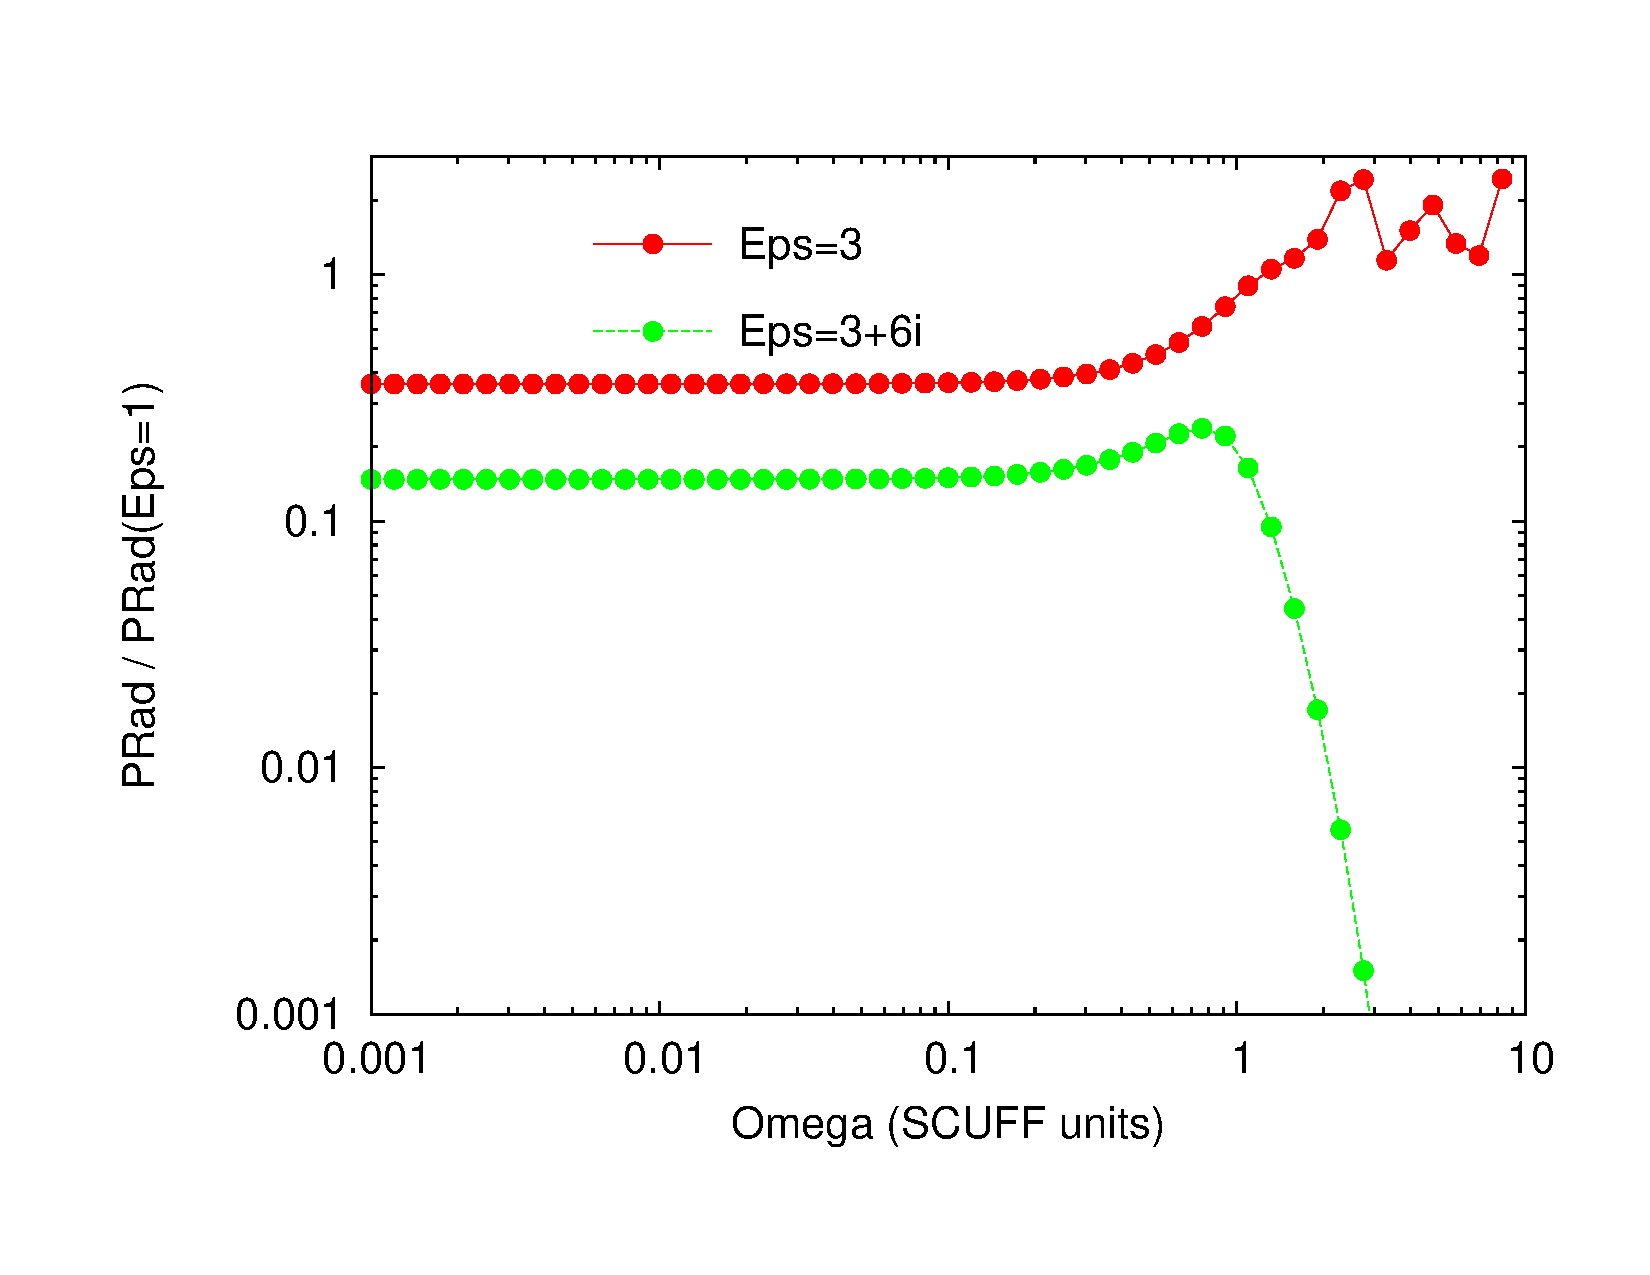
\includegraphics{PRadOverPRad0.pdf}}
\caption{Power radiated by a dipole at the center of a dielectric
sphere, normalized by the power radiated by a dipole in free space.}
\end{center}
\end{figure}
%####################################################################%

%%%%%%%%%%%%%%%%%%%%%%%%%%%%%%%%%%%%%%%%%%%%%%%%%%%%%%%%%%%%%%%%%%%%%%
%%%%%%%%%%%%%%%%%%%%%%%%%%%%%%%%%%%%%%%%%%%%%%%%%%%%%%%%%%%%%%%%%%%%%%
%%%%%%%%%%%%%%%%%%%%%%%%%%%%%%%%%%%%%%%%%%%%%%%%%%%%%%%%%%%%%%%%%%%%%%
\subsection{Sample stress-tensor force calculation}

The simplest incident-field configuration that gives rise to a
nonvanishing total force on the sphere is a superposition of 
$(1,0)$ and $(2,1)$ spherical waves, corresponding to coherent
dipole and quadrupole sources at the origin. Thus, in the
incident-field expansion (\ref{EIncExpansion}) we take
%%%%%%%%%%%%%%%%%%%%%%%%%%%%%%%%%%%%%%%%%%%%%%%%%%%%%%%%%%%%%%%%%%%%%%
\numeq{TwoNonvanishingPs}
{
 P_{(1,0)}=P_{(2,1)}=1,
 \qquad 
 P_\alpha=0 \text{ for all other }\alpha, 
 \qquad 
 Q_\alpha=0 \text{ for all }\alpha.
}
%%%%%%%%%%%%%%%%%%%%%%%%%%%%%%%%%%%%%%%%%%%%%%%%%%%%%%%%%%%%%%%%%%%%%%
The coefficients in expansions (\ref{EOutExpansion}, 
\ref{HOutExpansion}) for the fields outside the sphere 
are then similarly given by 
\numeq{TwoNonvanishingPs}
{
 C_{(1,0)}=C_{(2,1)}=\text{nonzero},
 \qquad 
 C_\alpha=0 \text{ for all other }\alpha, 
 \qquad 
 D_\alpha=0 \text{ for all }\alpha.
}
The actual values of $C_{(1,0)}$ and $C_{(2,1)}$, which
are less important for our immediate goals, are determined
by equation (\ref{CDAlpha}) for a specific frequency,
dielectric constant, and sphere radius. For example, 
for the particular case 
$\{ \omega, r_0, \epsilon\}
 =
 \{ \text{3 $\cdot$ 10$^{14}$ rad/sec},
    1\text{ $\mu$m},
    10
\}$
we find
$$ C_{(1,0)}=-0.558 + 0.760i, \qquad
   C_{(2,1)}= 0.100 + 0.001i.
$$

%%%%%%%%%%%%%%%%%%%%%%%%%%%%%%%%%%%%%%%%%%%%%%%%%%%%%%%%%%%%%%%%%%%%%%
%%%%%%%%%%%%%%%%%%%%%%%%%%%%%%%%%%%%%%%%%%%%%%%%%%%%%%%%%%%%%%%%%%%%%%
%%%%%%%%%%%%%%%%%%%%%%%%%%%%%%%%%%%%%%%%%%%%%%%%%%%%%%%%%%%%%%%%%%%%%%
\subsection{$x$-directed force density}

At a point $\vb x=(r_b, \Omega)$ on the surface of the bounding sphere
of radius $r_b$, the $x$-directed force per unit area is, from
(\ref{XForceFromEH}),
%====================================================================%
\begin{align*}
f_x(\vb x)
=\frac{\epsilon}{4}
  \bigg\{  &C^*_{10} C_{10} 
            \Big[ \vb M_{10}^*(\vb x) \bmc F_x(\Omega) \vb M_{10}(\vb x) 
                  + \vb N_{10}^*(\vb x) \bmc F_x(\Omega) \vb N_{10}(\vb x) 
            \Big]
\\
          +&C^*_{10} C_{21} 
            \Big[ \vb M_{10}^*(\vb x) \bmc F_x(\Omega) \vb M_{21}(\vb x) 
                  + \vb N_{10}^*(\vb x) \bmc F_x(\Omega) \vb N_{21}(\vb x)
            \Big]
\\
          +&C^*_{21} C_{10} 
            \Big[ \vb M_{21}^*(\vb x) \bmc F_x(\Omega) \vb M_{10}(\vb x) 
                  + \vb N_{21}^*(\vb x) \bmc F_x(\Omega) \vb N_{10}(\vb x)
            \Big]
\\
          +&C^*_{21} C_{21} 
            \Big[ \vb M_{21}^*(\vb x) \bmc F_x(\Omega) \vb M_{21}(\vb x) 
                  + \vb N_{21}^*(\vb x) \bmc F_x(\Omega) \vb N_{21}(\vb x)
            \Big]
  \bigg\}
\end{align*}
%====================================================================%

%%%%%%%%%%%%%%%%%%%%%%%%%%%%%%%%%%%%%%%%%%%%%%%%%%%%%%%%%%%%%%%%%%%%%%
%%%%%%%%%%%%%%%%%%%%%%%%%%%%%%%%%%%%%%%%%%%%%%%%%%%%%%%%%%%%%%%%%%%%%%
%%%%%%%%%%%%%%%%%%%%%%%%%%%%%%%%%%%%%%%%%%%%%%%%%%%%%%%%%%%%%%%%%%%%%%
\subsection{Total $x$-directed force}

The \textit{total} force is obtained from equation (\ref{TotalForce}):
\begin{equation}
 F_x = 
\frac{\epsilon_0}{4}
 \bigg\{
       C_{10}^* C_{21}
       \Big[ \Vmv{\vb M_{10}}{\bmc F_x}{\vb M_{21}}
            +\Vmv{\vb N_{10}}{\bmc F_x}{\vb N_{21}}
       \Big]
       + \text{CC}
 \bigg\}
\label{TotalForce2}
\end{equation}
where \text{CC} stands for ``complex conjugate.''
[The inner product here is defined by equation 
 (\ref{InnerProductDefinition}).]
With some effort, we compute
%%%%%%%%%%%%%%%%%%%%%%%%%%%%%%%%%%%%%%%%%%%%%%%%%%%%%%%%%%%%%%%%%%%%%%
$$
 \Vmv{\vb M_{10}}{\bmc F_x}{\vb M_{21}}
      +\Vmv{\vb N_{10}}{\bmc F_x}{\vb N_{21}}
 =-i\sqrt\frac{3}{10} \frac{1}{k^2}
$$
%%%%%%%%%%%%%%%%%%%%%%%%%%%%%%%%%%%%%%%%%%%%%%%%%%%%%%%%%%%%%%%%%%%%%%
and thus the total force (\ref{TotalForce2}) reads
\numeq{FxFinalSpecialCase}
{
 F_x = -\frac{\epsilon_0}{2k^2}\sqrt\frac{3}{10}\text{ Im }\Big(C_{10}^* C_{21}\Big)
}
%%%%%%%%%%%%%%%%%%%%%%%%%%%%%%%%%%%%%%%%%%%%%%%%%%%%%%%%%%%%%%%%%%%%%%
To make sense of the units here, suppose that field-strength
coefficients like $P,Q,C,D$ in (\ref{EIncExpansion}) and 
(\ref{EOutExpansion}) are measured in typical {\sc scuff-em}
units of V/$\mu $m, while $k$ is measured in units of 
inverse $\mu m$. Then the units of (\ref{FxFinalSpecialCase}) are

%%%%%%%%%%%%%%%%%%%%%%%%%%%%%%%%%%%%%%%%%%%%%%%%%%%%%%%%%%%%%%%%%%%%%%
\begin{align*}
 \text{units of (\ref{FxFinalSpecialCase})}
&=\frac{\epsilon_0 \cdot \text{V}^2 \cdot \mu\text{m}^{-2}}{\mu \text{m}^{-2}}
\intertext{Use $\epsilon_0=\frac{1}{Z_0 c}$ where $c$ is 
           the vacuum speed of light:}
&=\frac{1}{Z_0 c}\cdot \text{V}^2
\intertext{Use $Z_0=376.7$ V/A:}
&= \frac{ 376.7 \text{ V $\cdot$ A} }
        { 3\cdot 10^{14} \, \mu\text{m} \cdot \text{s}^{-1}}
\intertext{Now use 1 V$\cdot$ A=1 watt, 1 watt $\cdot$ 1 s = 1 joule,
           1 joule / 1 $\mu$m = 10$^6$ Newtons:}
&=1.26\cdot 10^{-6} \text{ Newtons.}
\end{align*}

%####################################################################%
\begin{figure}[H]
\begin{center}
\resizebox{\textwidth}{!}{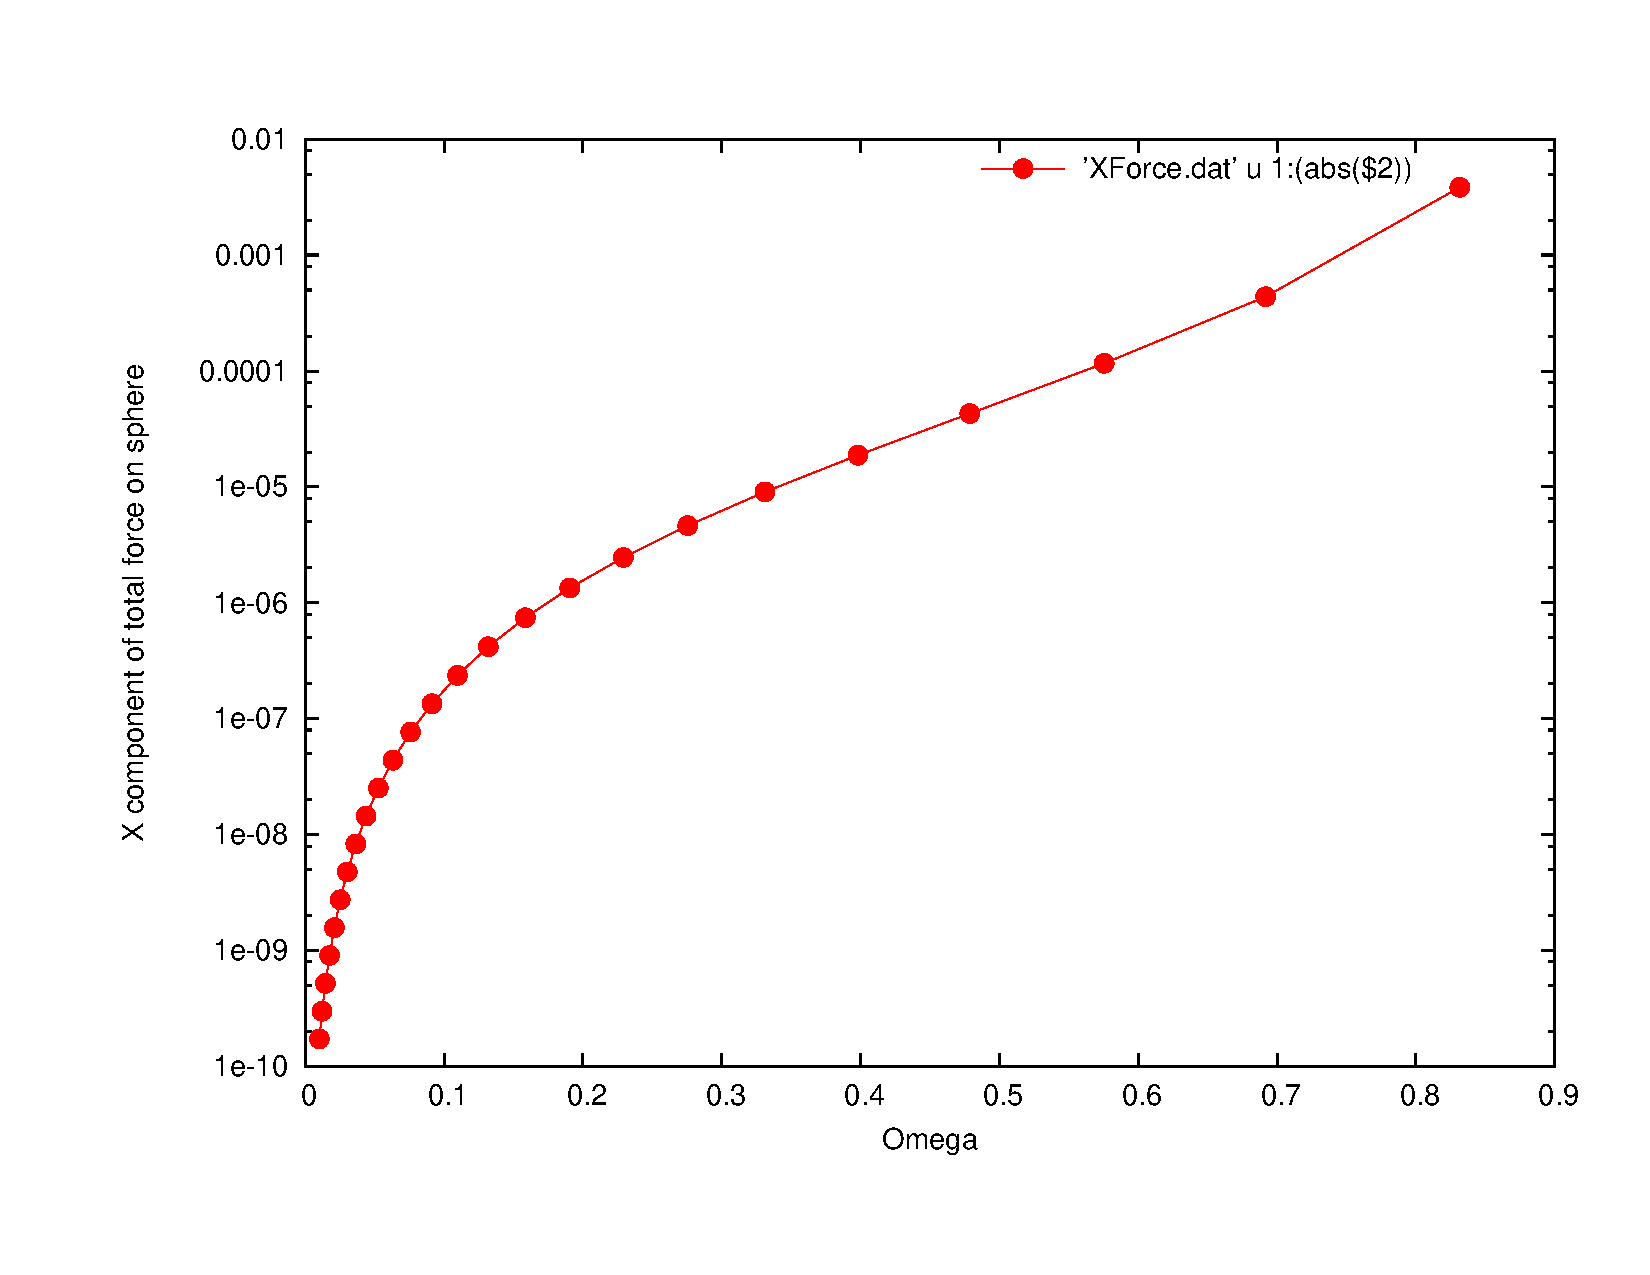
\includegraphics{ExactForce.pdf}}
\caption{$x$-component of total force on sphere irradiated from 
         within by an incident field of the form (\ref{EIncExpansion}) 
         with coefficients (\ref{TwoNonvanishingPs}).
        }
\label{TotalForce}
\end{center}
\end{figure}

\end{document}
